\documentclass[11pt]{article}
\usepackage[margin=1in]{geometry}
\usepackage{graphicx}
\usepackage{subcaption}
\usepackage{float}
\usepackage{amsmath}
\usepackage{enumitem}

\title{EE 168: Introduction to VLSI\\Homework 2}
\author{Kaushik Vada}

\begin{document}

\maketitle

\section*{Problem 1: Static CMOS Gate Design}
Design the static complementary gates (CMOS gates) for the following logic expressions using pull-up/pull-down networks. Use a truth table to show logical equivalence for converted expressions. Assume inverted variables are available, i.e., you do not have to add inverters for complementary variables.

\begin{enumerate}[label={\bfseries\alph*)}, itemsep=1em]
    \item
    \begin{figure}[H]
        \centering
        \begin{subfigure}{0.47\textwidth}
            \centering
            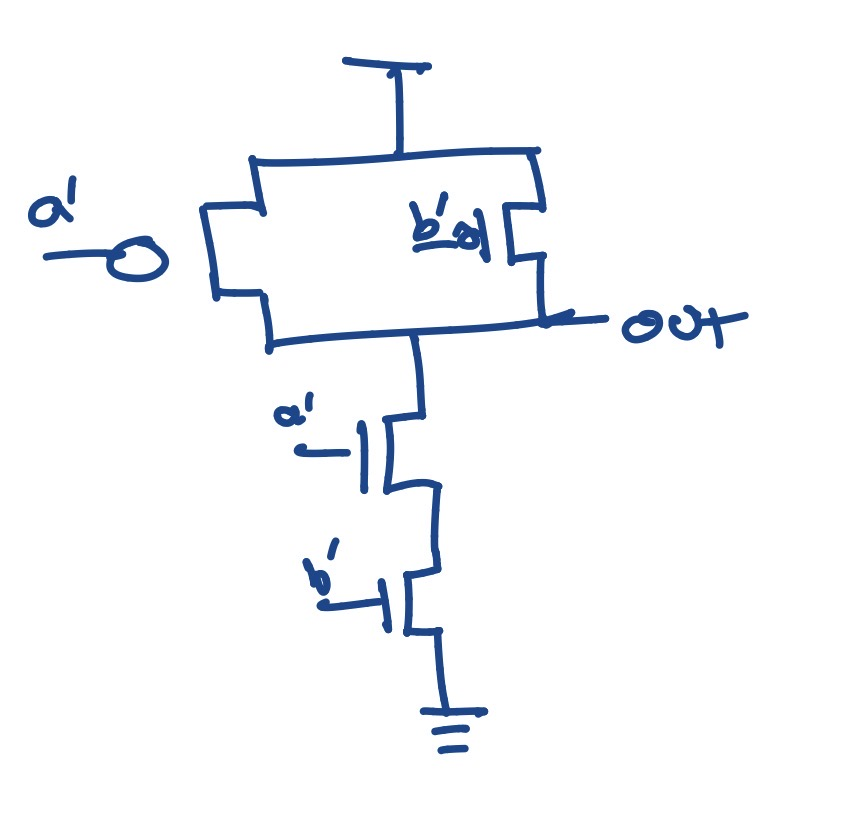
\includegraphics[width=\linewidth]{question1/1a.jpeg}
        \end{subfigure}
        \hfill
        \begin{subfigure}{0.47\textwidth}
            \centering
            {\renewcommand{\arraystretch}{1.25}%
            \setlength{\tabcolsep}{6pt}%
            \resizebox{\linewidth}{!}{%
            \begin{tabular}{ccccc}
                \multicolumn{5}{c}{\(a + b = (a' \cdot b')'\)} \\
                \hline
                \(ab\) & \(a'b'\) & \(a' \cdot b'\) & \((a' \cdot b')'\) & \(a + b\) \\
                \hline
                00 & 11 & 1 & 0 & 0 \\
                01 & 10 & 0 & 1 & 1 \\
                10 & 01 & 0 & 1 & 1 \\
                11 & 00 & 0 & 1 & 1 \\
                \hline
            \end{tabular}}%
            }
        \end{subfigure}
    \end{figure}

    \item
    \begin{figure}[H]
        \centering
        \begin{subfigure}{0.47\textwidth}
            \centering
            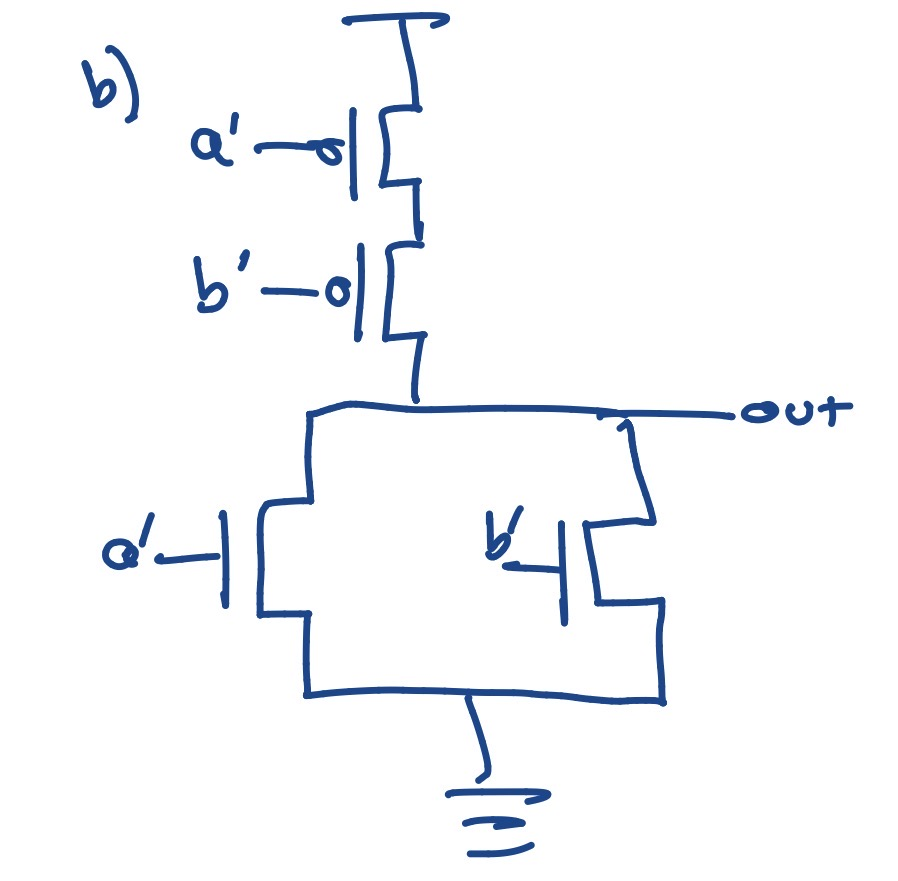
\includegraphics[width=\linewidth]{question1/1b.jpeg}
        \end{subfigure}
        \hfill
        \begin{subfigure}{0.47\textwidth}
            \centering
            {\renewcommand{\arraystretch}{1.25}%
            \setlength{\tabcolsep}{6pt}%
            \resizebox{\linewidth}{!}{%
            \begin{tabular}{ccccc}
                \multicolumn{5}{c}{\(ab = (a' + b')'\)} \\
                \hline
                \(ab\) & \(a'b'\) & \(a' + b'\) & \((a' \cdot b')'\) & \(a + b\) \\
                \hline
                00 & 11 & 1 & 0 & 0 \\
                01 & 10 & 1 & 0 & 0 \\
                10 & 01 & 1 & 0 & 0 \\
                11 & 00 & 0 & 1 & 1 \\
                \hline
            \end{tabular}}%
            }
        \end{subfigure}
    \end{figure}

    \item
    \begin{figure}[H]
        \centering
        \begin{subfigure}{0.47\textwidth}
            \centering
            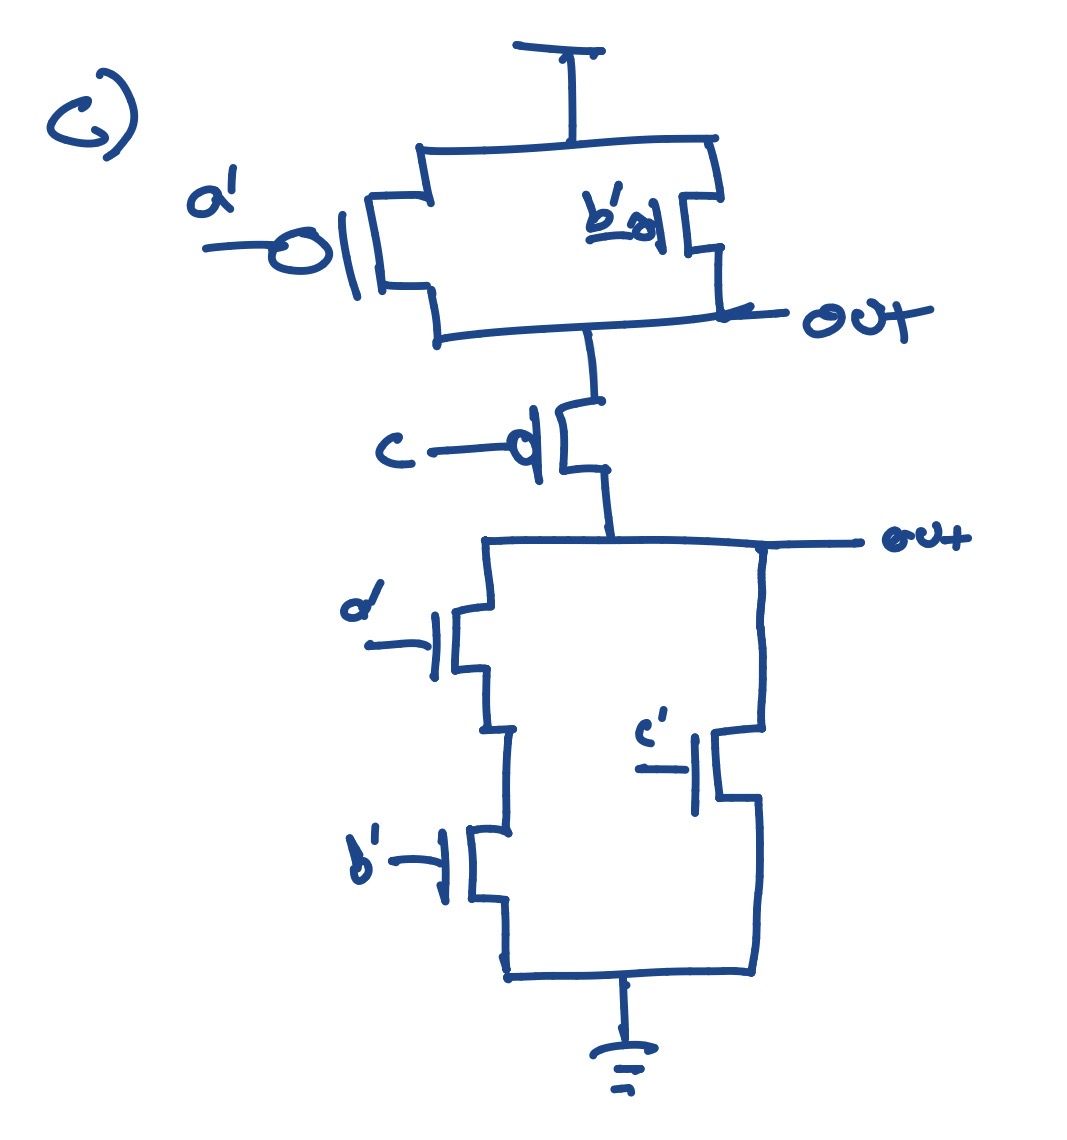
\includegraphics[width=\linewidth]{question1/1c.jpeg}
        \end{subfigure}
        \hfill
        \begin{subfigure}{0.47\textwidth}
            \centering
            {\renewcommand{\arraystretch}{1.2}%
            \setlength{\tabcolsep}{6pt}%
            \resizebox{\linewidth}{!}{%
            \begin{tabular}{cccccc}
                \multicolumn{6}{c}{\((a + b)c = ((a + b)' + c')' = ((a' \cdot b') + c')'\)} \\
                \hline
                \(abc\) & \(a'b'c'\) & \(a' \cdot b'\) & \((a' \cdot b') + c'\) & \(((a' \cdot b') + c')'\) & \((a + b)c\) \\
                \hline
                000 & 111 & 1 & 1 & 0 & 0 \\
                001 & 110 & 1 & 1 & 0 & 0 \\
                010 & 101 & 0 & 1 & 0 & 0 \\
                011 & 100 & 0 & 0 & 1 & 1 \\
                100 & 011 & 0 & 1 & 0 & 0 \\
                101 & 010 & 0 & 0 & 1 & 1 \\
                110 & 001 & 0 & 1 & 0 & 0 \\
                111 & 000 & 0 & 0 & 1 & 1 \\
                \hline
            \end{tabular}}%
            }
        \end{subfigure}
    \end{figure}

    \item
    \begin{figure}[H]
        \centering
        \begin{subfigure}{0.47\textwidth}
            \centering
            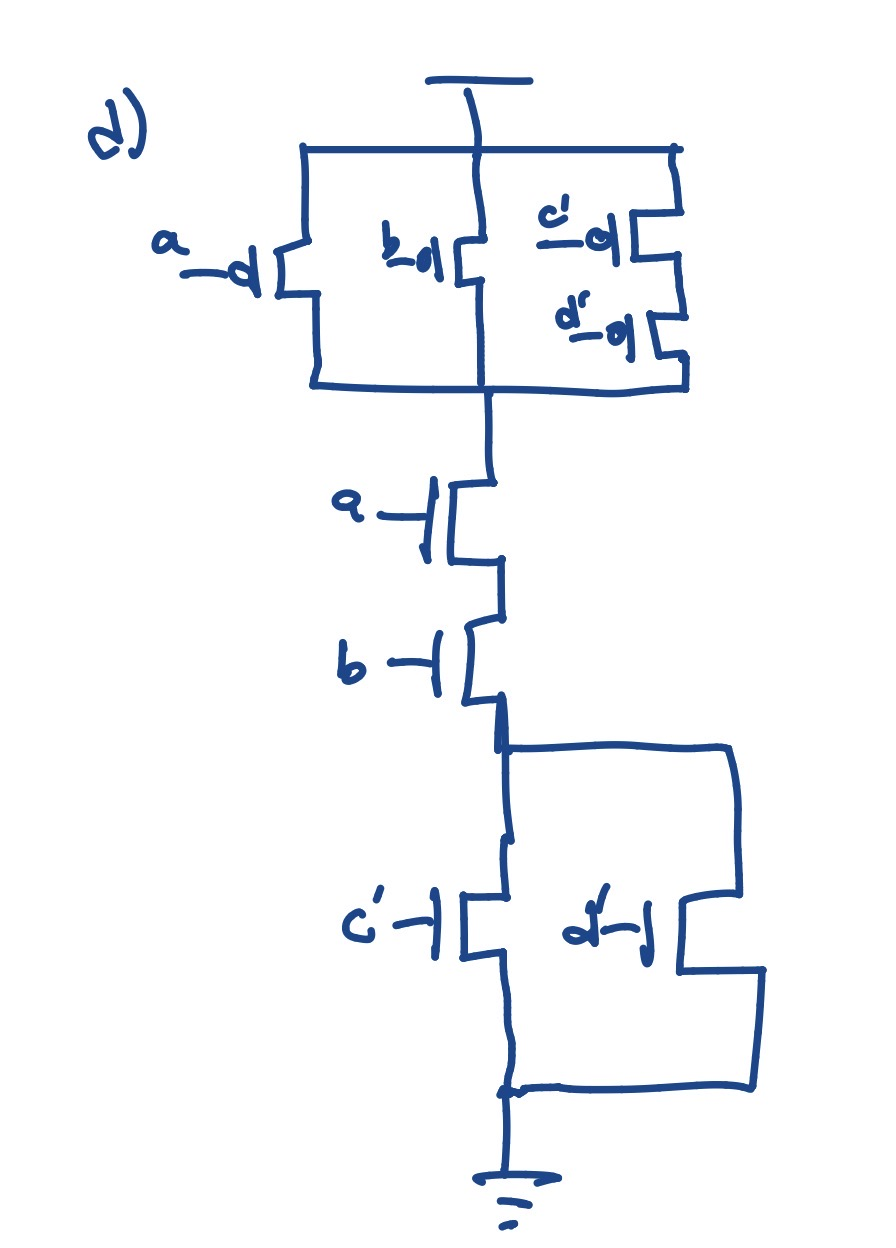
\includegraphics[width=\linewidth]{question1/1d.jpeg}
        \end{subfigure}
        \hfill
        \begin{subfigure}{0.47\textwidth}
            \centering
            {\renewcommand{\arraystretch}{1.15}%
            \setlength{\tabcolsep}{6pt}%
            \resizebox{\linewidth}{!}{%
            \begin{tabular}{cccccc}
                \multicolumn{6}{c}{\((ab)' + (cd) = (ab \cdot (c' + d'))'\)} \\
                \hline
                \(abcd\) & \(ab\) & \(c'd'\) & \(c' + d'\) & \(ab \cdot (c' + d')\) & \((ab \cdot (c' + d'))'\) \\
                \hline
                0000 & 0 & 11 & 1 & 0 & 1 \\
                0001 & 0 & 10 & 1 & 0 & 1 \\
                0010 & 0 & 01 & 1 & 0 & 1 \\
                0011 & 0 & 00 & 0 & 0 & 1 \\
                0100 & 0 & 11 & 1 & 0 & 1 \\
                0101 & 0 & 10 & 1 & 0 & 1 \\
                0110 & 0 & 01 & 1 & 0 & 1 \\
                0111 & 0 & 00 & 0 & 0 & 1 \\
                1000 & 0 & 11 & 1 & 0 & 1 \\
                1001 & 0 & 10 & 1 & 0 & 1 \\
                1010 & 0 & 01 & 1 & 0 & 1 \\
                1011 & 0 & 00 & 0 & 0 & 1 \\
                1100 & 1 & 11 & 1 & 1 & 0 \\
                1101 & 1 & 10 & 1 & 1 & 0 \\
                1110 & 1 & 01 & 1 & 1 & 0 \\
                1111 & 1 & 00 & 0 & 0 & 1 \\
                \hline
            \end{tabular}}%
            }
        \end{subfigure}
\end{figure}
\end{enumerate}
\newpage
\section*{Problem 2: Complex Gate Implementations}
Write the defining logic expressions and draw the transistor level schematic for each complex gate below.

\begin{enumerate}[label={\bfseries\alph*)}, itemsep=1em]
    \item 
    \begin{center}
        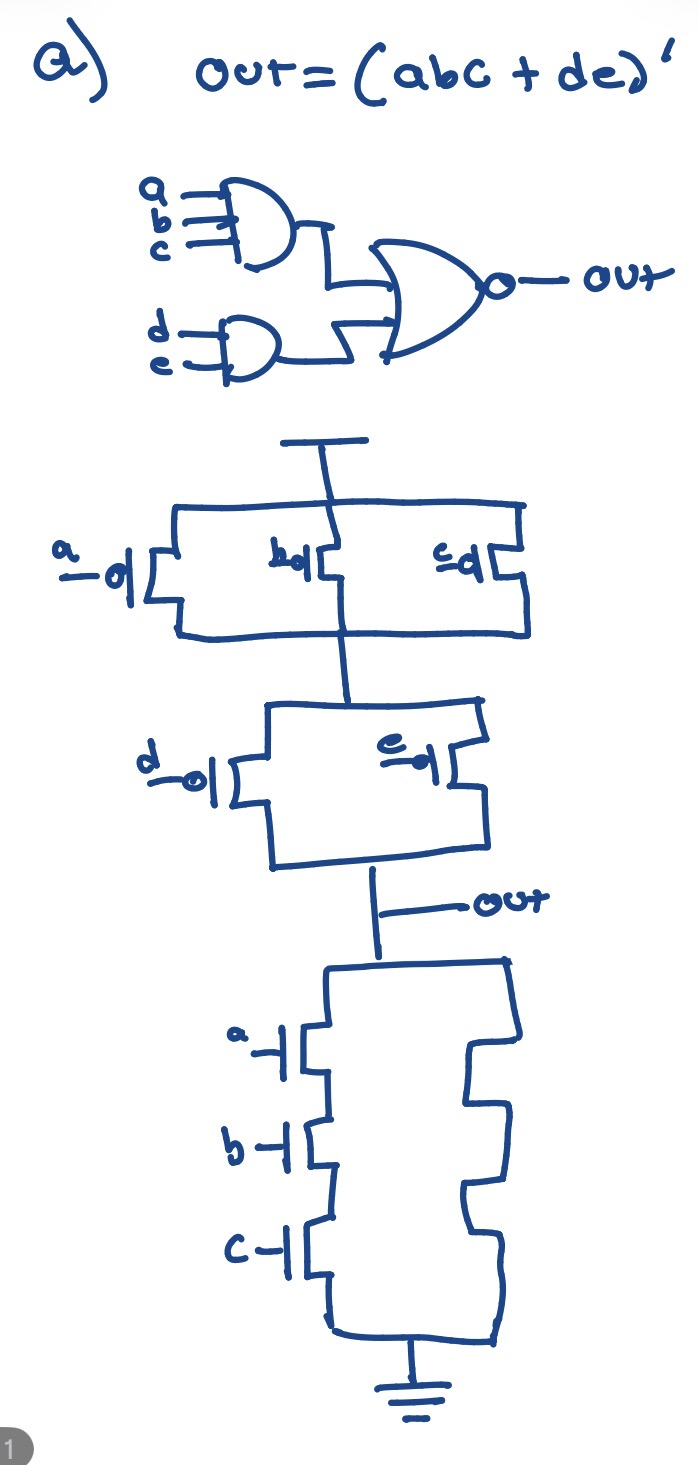
\includegraphics[width=0.4\textwidth]{question2/2a.jpeg}
    \end{center}

    \item 
    \begin{center}
        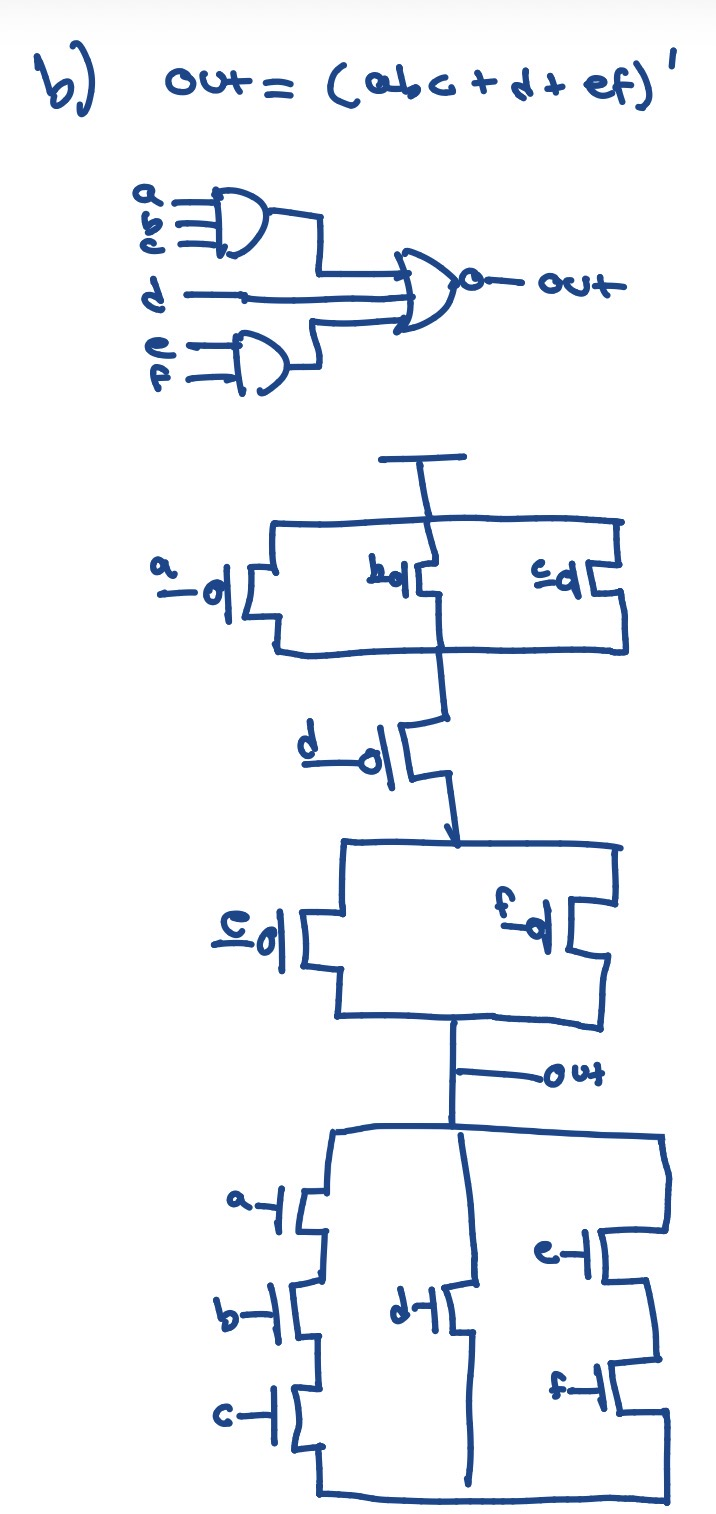
\includegraphics[width=0.4\textwidth]{question2/2b.jpeg}
    \end{center}

    \item 
    \begin{center}
        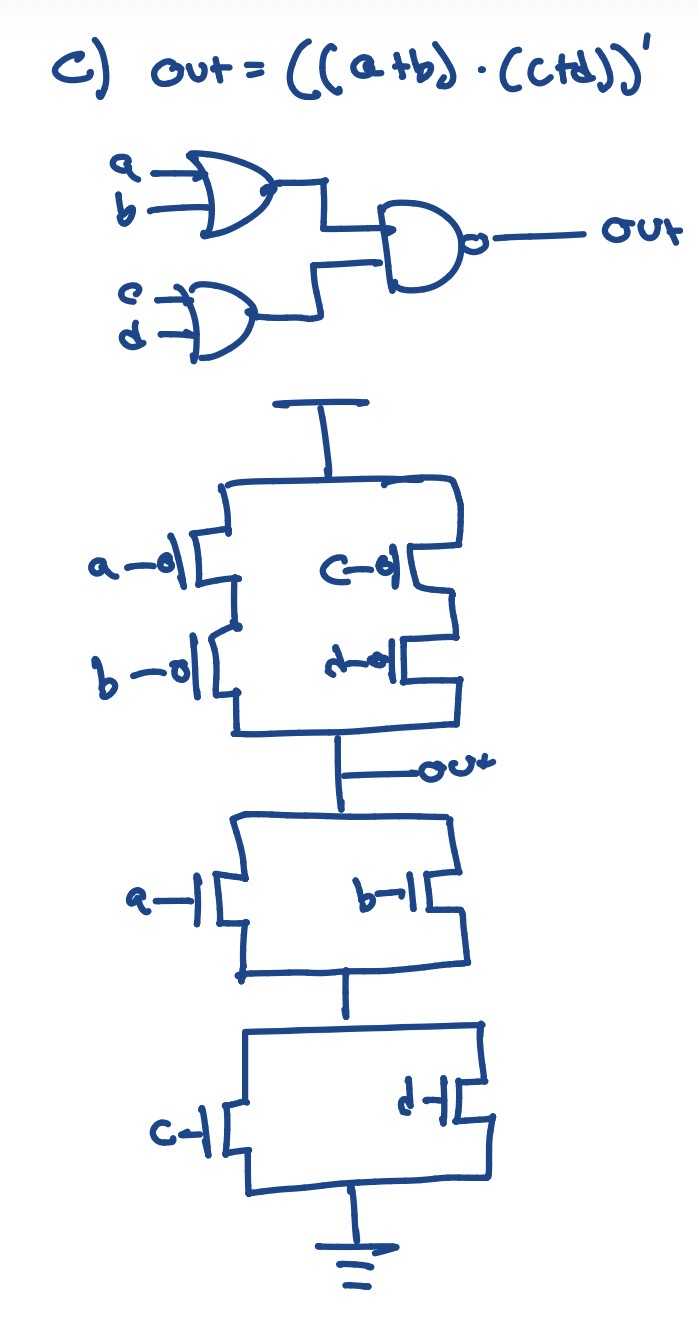
\includegraphics[width=0.4\textwidth]{question2/2c.jpeg}
    \end{center}

    \item 
    \begin{center}
        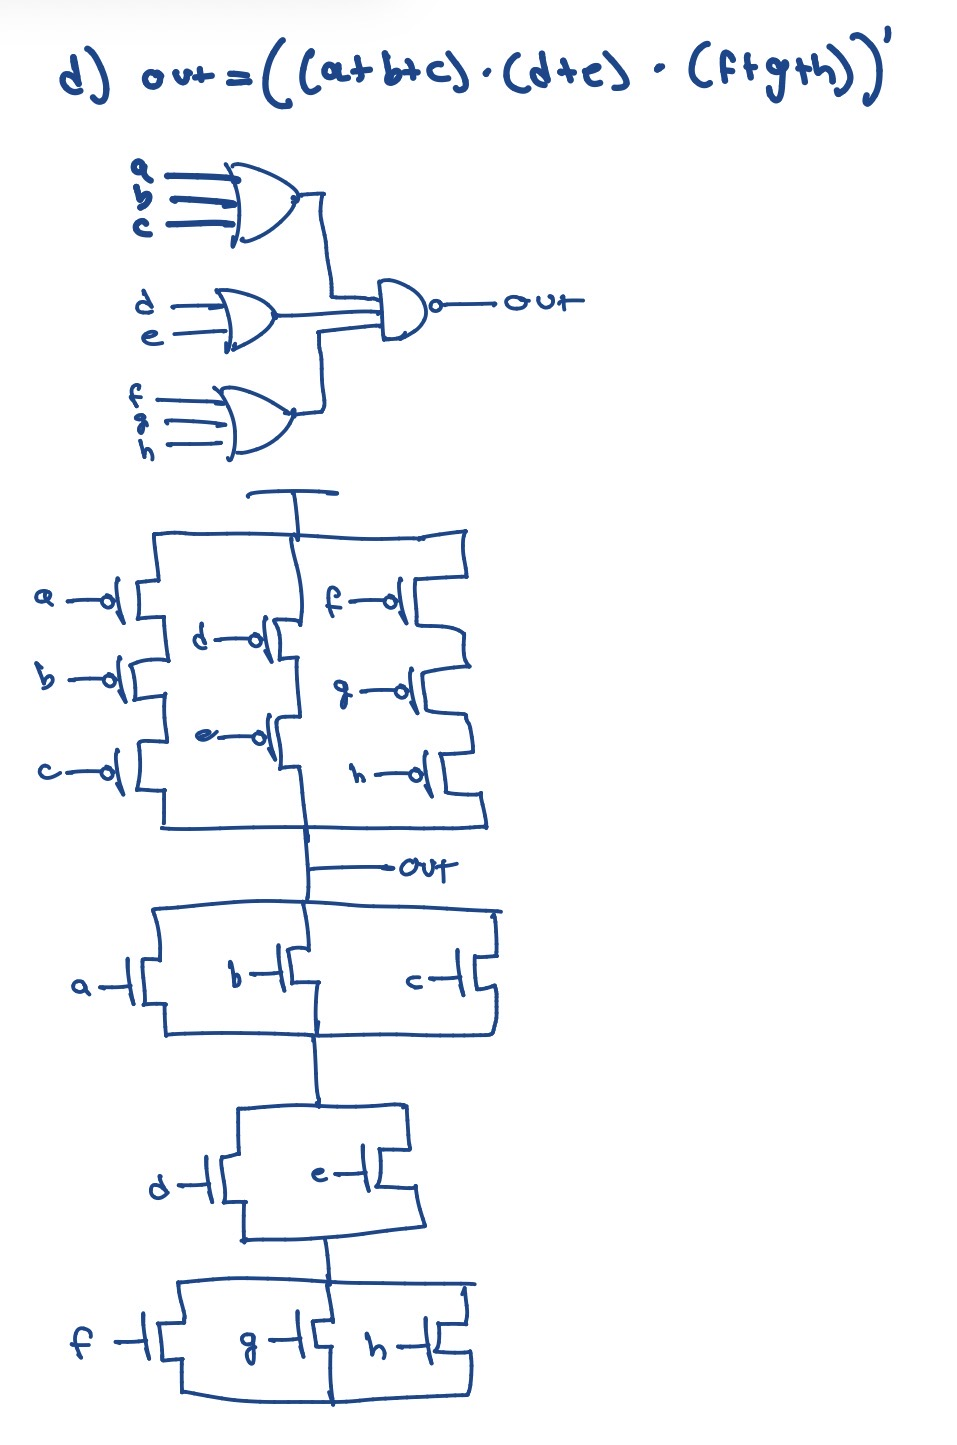
\includegraphics[width=0.4\textwidth]{question2/2d.jpeg}
    \end{center}
\end{enumerate}

\clearpage

\section*{Problem 5: Effective Resistance with Varying Load Capacitance}
Compute the value of \(R_{\text{eff}}\) required to model the behavior of an inverter that reaches 50\% of its output value at 20\text{ ps} with load \(C_L\) equal to \(3C_1\), \(4C_1\), and \(5C_1\). What effect does load capacitance have on the effective resistance? \((C_1 = 0.89\times 10^{-15})\)
\[
C_1 = 0.89\,\text{fF},\qquad t_s = 20\,\text{ps},\qquad \frac{V_f}{V_0} = 0.5
\]
\[
R_{\text{eff}} = \frac{t_s}{C_L \ln \left( \frac{V_f}{V_0} \right)}
\]
\[
C_L = 3C_1 \implies R_{\text{eff}} = \frac{20\times10^{-12}}{3 \times 0.89 \times 10^{-15} \ln(0.5)} = 1.081\times10^{4}\,\Omega = 10.81\,\text{k}\Omega
\]
\[
C_L = 4C_1 \implies R_{\text{eff}} = \frac{20\times10^{-12}}{4 \times 0.89 \times 10^{-15} \ln(0.5)} = 8.11\times10^{3}\,\Omega = 8.11\,\text{k}\Omega
\]
\[
C_L = 5C_1 \implies R_{\text{eff}} = \frac{20\times10^{-12}}{5 \times 0.89 \times 10^{-15} \ln(0.5)} = 6.48\times10^{3}\,\Omega = 6.48\,\text{k}\Omega
\]
\[
\text{Larger } C_L \Rightarrow \text{smaller } R_{\text{eff}}.
\]

\clearpage

\section*{Problem 6: Transition Times for Four-Input NAND Driving NOR Gate}
Compute transition times for a four-input NAND gate with 8/2 pulldown (the \(W/L = 8/2\) for n-type transistors) and 8/2 pullup that drives an identically sized NOR four-input gate (the NAND gate only drives one input of the NOR gate).
\begin{center}
    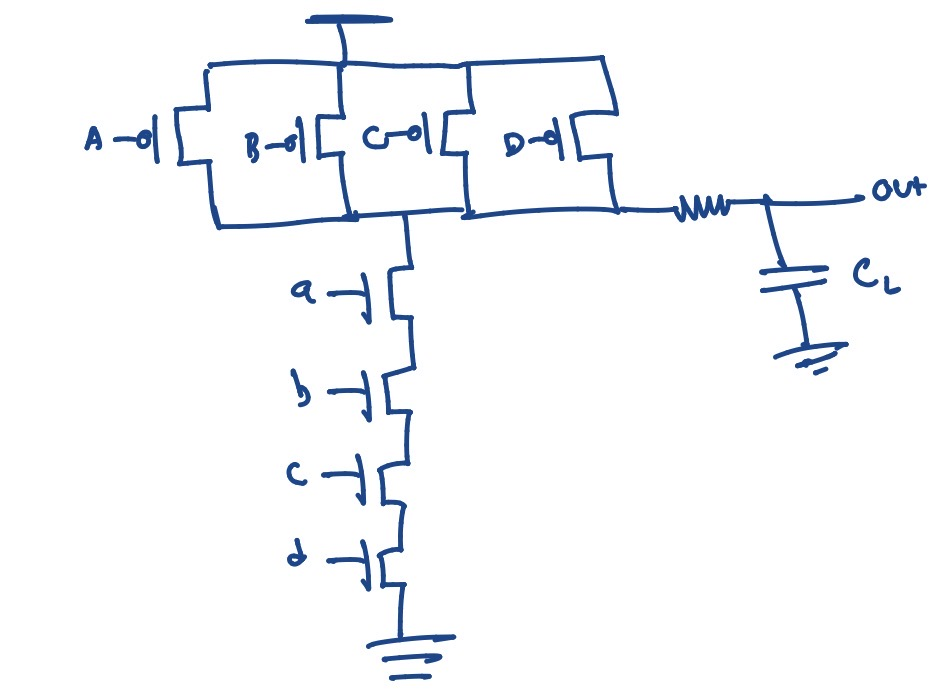
\includegraphics[width=0.6\textwidth]{question6/6.jpeg}
\end{center}
\[
R_{\text{up}} = 1 \cdot \frac{L_p}{W_p} \cdot R_p = 1 \times \frac{2}{8} \times 29.6 = 7.40\,\text{k}\Omega
\]
\[
R_{\text{down}} = 4 \cdot \frac{L_n}{W_n} \cdot R_n = 4 \times \frac{2}{8} \times 6.47 = 6.47\,\text{k}\Omega
\]
\[
R_L = 0,\qquad C_L = \left(\frac{W_p}{L_p} + \frac{W_n}{L_n}\right) C_1 = \left(\frac{8}{2} + \frac{8}{2}\right) \cdot 0.89\times10^{-15} = 7.12\,\text{fF}
\]
\[
t_r = -(R_{\text{up}} + R_L) C_L \ln(0.1) = -7.40\times10^3 \cdot 7.12\times10^{-15} \ln(0.1) = 121.32\,\text{ps}
\]
\[
t_f = -(R_{\text{down}} + R_L) C_L \ln(0.1) = -6.47\times10^3 \cdot 7.12\times10^{-15} \ln(0.1) = 106.07\,\text{ps}
\]

\clearpage

\section*{Problem 7: Rise Time with Different Interconnects}
Compute rise time for a two-input NAND gate with 8/2 pull-down and 8/2 pull-up that drives the interconnects described below (assume the wire impedance is modeled as a single lump):
\[
R_{\text{up}} = 1 \cdot \frac{L_p}{W_p} \cdot R_p = 1 \times \frac{2}{8} \times 29.6 = 7.4\,\text{k}\Omega,\qquad \lambda = \frac{180}{2} = 90\,\text{nm} = 0.09\,\mu\text{m}
\]
\[
A = WL,\qquad P = 2(W + L)
\]
\begin{enumerate}[label={\bfseries\alph*)}, itemsep=2ex]
    \item Poly interconnect ($W = 3\lambda,\, L = 300\lambda$):
    \begin{align*}
    R_L &= 8\frac{L}{W} = 8\frac{3000\lambda}{3\lambda} = 800~\Omega,\\
    C_L &= 63\times10^{-18}\big(27\cdot0.27 + 2(27 + 0.27)\big) = 3.90\times10^{-15}\,\text{F},\\
    t_r &= -\big(7.4\times10^{3} + 800\big)\,C_L\,\ln 0.1 = 73.55~\text{ps}.
    \end{align*}

    \item Metal-1 interconnect ($W = 4\lambda,\, L = 600\lambda$):
    \begin{align*}
    R_L &= 0.08\frac{L}{W} = 0.08\frac{600\lambda}{4\lambda} = 12~\Omega,\\
    C_L &= 36\times10^{-18}(54\cdot0.36) + 54\times10^{-18}\,2(54 + 0.36) = 6.57\times10^{-15}\,\text{F},\\
    t_r &= -\big(7.4\times10^{3} + 12\big)\,C_L\,\ln 0.1 = 111.98~\text{ps}.
    \end{align*}

    \item Metal-2 interconnect ($W = 4\lambda,\, L = 1200\lambda$):
    \begin{align*}
    R_L &= 0.08\frac{L}{W} = 0.08\frac{1200\lambda}{4\lambda} = 24~\Omega,\\
    C_L &= 36\times10^{-18}(108\cdot0.36) + 51\times10^{-18}\,2(108 + 0.36) = 1.245\times10^{-14}\,\text{F},\\
    t_r &= -\big(7.4\times10^{3} + 24\big)\,C_L\,\ln 0.1 = 212.25~\text{ps}.
    \end{align*}
\end{enumerate}

\clearpage

\section*{Problem 8: Buffer Insertion Delay Optimization}
For a metal 1 wire with \(R_{\text{int}} = 500\,\Omega\), \(C_{\text{int}} = 200\,\text{fF}\), and minimum-size buffer parameters \(R_0 = 6.47\,\text{k}\Omega\) and \(C_0 = 1.78\,\text{fF}\), determine the 50\% delay in the following cases:
\begin{enumerate}[label={\bfseries\alph*)}, itemsep=2ex]
    \item One buffer inserted, one section \((k = 1)\), buffers at minimum size \((h = 1)\).
    \item Two buffers inserted, wire divided into two sections \((k = 2)\), buffers at minimum size \((h = 1)\).
    \item Two buffers inserted, wire divided into two sections \((k = 2)\), buffers sized to twice minimum \((h = 2)\).
    \item Optimal number of buffers, buffer size, and the resulting minimum 50\% delay.
\end{enumerate}

\[
T_{50\%}(k,h) = k \Bigg[0.7 \frac{R_0}{h} \Big(\frac{C_{\text{int}}}{k} + h C_0 \Big) + R_{\text{int}} \Big(0.4 \frac{C_{\text{int}}}{k} + 0.7 h C_0 \Big) \Bigg]
\]

\begin{enumerate}[label=\bfseries\alph*), itemsep=2ex]
    \item Minimum-size single buffer ($k=1, h=1$):
    \begin{align*}
    \alpha &= 0.7 R_0 = 4.529\times10^{3}\,\Omega,\\
    C_{\Sigma} &= C_{\text{int}} + C_0 = 201.78\times10^{-15}\,\text{F},\\
    \beta &= 0.4 C_{\text{int}} + 0.7 C_0 = 81.246\times10^{-15}\,\text{F},\\
    T_{50\%} &= \alpha C_{\Sigma} + R_{\text{int}} \beta = 9.5448\times10^{-10}\,\text{s} = 954.48~\text{ps}.
    \end{align*}

    \item Two sections with minimum buffers ($k=2, h=1$):
    \begin{align*}
    C_{\text{stage}} &= \frac{C_{\text{int}}}{2} + C_0 = 101.78\times10^{-15}\,\text{F},\\
    \beta_{\text{stage}} &= 0.4\frac{C_{\text{int}}}{2} + 0.7 C_0 = 41.246\times10^{-15}\,\text{F},\\
    T_{50\%} &= 2\Big[\alpha C_{\text{stage}} + \frac{R_{\text{int}}}{2} \beta_{\text{stage}}\Big] = 9.4255\times10^{-10}\,\text{s} = 942.55~\text{ps}.
    \end{align*}

    \item Two sections with buffers twice minimum ($k=2, h=2$):
    \begin{align*}
    \alpha_2 &= 0.7 \frac{R_0}{2} = 2.2645\times10^{3}\,\Omega,\\
    C_{\text{stage}} &= \frac{C_{\text{int}}}{2} + 2 C_0 = 103.56\times10^{-15}\,\text{F},\\
    \beta_{\text{stage}} &= 0.4\frac{C_{\text{int}}}{2} + 0.7 (2 C_0) = 42.492\times10^{-15}\,\text{F},\\
    T_{50\%} &= 2\Big[\alpha_2 C_{\text{stage}} + \frac{R_{\text{int}}}{2} \beta_{\text{stage}}\Big] = 4.9027\times10^{-10}\,\text{s} = 490.27~\text{ps}.
    \end{align*}

    \item Optimal buffering:
    \begin{align*}
    k_{\text{opt}} &= \sqrt{\frac{0.4 R_{\text{int}} C_{\text{int}}}{0.7 R_0 C_0}} = 2.23,\\
    h_{\text{opt}} &= \frac{R_0 C_{\text{int}}}{R_{\text{int}} C_0} = 38.13,\\
    T_{50\%}^{\text{min}} &= 2.5 \sqrt{R_0 C_0 R_{\text{int}} C_{\text{int}}} = 8.484\times10^{-11}\,\text{s} = 84.84~\text{ps}.
    \end{align*}
\end{enumerate}



\end{document}
